\documentclass{mbd_fullpaper}

\begin{document}

%New commands
\newcommand{\heading}[1]{
   {\medskip\hskip5em\bf\large{#1}
   \vskip0.5ex
   }
}
\newcommand{\eqnref}[1]{
  (\ref{#1})
}

\renewcommand{\refname}{\medskip\bf\large References}



%------------------------------------------------------------
% title
\begin{center}
  \Large{\bf
Equivalent Mass-Spring Models of Multibody Spacecraft for the Application of Wave-based Control  }
\end{center}

%------------------------------------------------------------
% authors
\begin{center}
\large{
Joseph Thompson
}
\end{center}

%------------------------------------------------------------
% affiliations
{
\begin{center}
 \small
  \begin{tabular}{c}
    School of Mechanical and Materials Engineering \\
    University College Dublin              \\
    Belfield, Dublin 4, Ireland        \\
    joseph.thompson@ucdconnect.ie                        \\
  \end{tabular}
\end{center}
}

%------------------------------------------------------------
% abstract



\section*{Abstract}

% 250 words max.
Wave-Based Control (WBC) is particularly effective for achieving rest to rest motion of under-actuated, cascaded, lumped flexible systems.
In this control scheme the actuator simultaneously launches and absorbs wave components travelling into and out of the system at one end.
By doing this the control scheme combines position control and active vibration damping.
Much work has been done on wave-based modelling and control of mass-spring strings.
This paper asks the question: to what extent can this work be extended to a wider class of systems?
This question is motivated by the control of spacecraft with features such as structural flexibility, flexible appendages and fuel slosh.
Most mathematical models of these systems presented to the control engineer, do not obviously have the structure of a mass-spring string.
However, often it is possible to calculate an equivalent mass-spring system.
This paper identifies a class of systems, with real, positive and distinct eigenvalues, for which this transformation is possible and presents an algorithm for calculating the equivalent mass and spring values.
A segmented planar multibody rocket model is used as an example.
This model consists of three rigid bodies connected by two torsional springs and a gimballed rocket engine with constant thrust which may be used for attitude control.
Several test cases with different sensor and actuator configurations are examined and equivalent mass-spring systems are calculated in each case.

\section{extended abs}

\heading{Abstract}
Wave-Based Control (WBC) is particularly effective for achieving rest to rest motion of under-actuated, cascaded, lumped flexible systems such as in Fig.~\ref{fig:rec_sys}. The motion of each mass $x_1$ to $x_n$ of this system can be considered as a superposition of rightwards and leftwards travelling components or ‘waves’, starting at the actuator $x_0$, travelling to the tip, $x_n$, and returning to the actuator. The control strategy is based on considering the motion of the actuator $x_0$ as simultaneously launching rightwards travelling motion (waves) into the system while absorbing leftwards travelling motion coming back from the system. For rest-to-rest manoeuvres to a target displacement, the controller launches a wave into the system of half the target displacement and absorbs the returning wave after it has travelled to the end of the system and has been reflected back to the actuator. This absorption by the actuator moves the system the second half of the target displacement while absorbing vibrations. Thus position control and active vibration damping are combined in a single actuator motion. The resulting control strategies have many advantages, including robustness to modelling errors and system changes, minimal sensing and ease of implementation.
%\begin{figure}[h]
%  \begin{center}
%    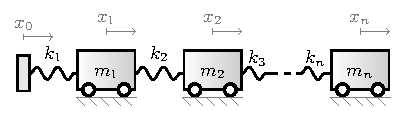
\includegraphics[scale=1]{lumped_system.pdf}
%    \caption{Non-uniform lumped system with one free and one moving boundary \label{fig:rec_sys}}
%  \end{center}
%\end{figure}
The cascaded system of Fig.~\ref{fig:rec_sys} is similar to a range of systems of practical engineering interest, including robot arms, cranes, space structures and disk drive heads. Much work has been done on wave-based modelling and control of such systems \cite{OConnor2011, Connor2005}. This paper asks the question: to what extent can this work be extended to a wider class of systems? 
This question is motivated by the control of spacecraft with features such as structural flexibility, flexible appendages and fuel slosh.
Mathematical models of these systems, as presented to the control engineer, do not appear to have the same structure as a mass-spring string actuated at one end.
Many systems for instance are modelled as multi-rigid-body systems ~\cite{Kane1980} with multiple sensors and actuators or simply presented as a linear system in the form of a set of state space matrices.
This leads to the following problem. Given a generic, SISO (single-input single-output), lightly damped mechanical system described by
\begin{equation}
\ddot{\mathbf{q}}(t) + \Lambda\mathbf{q}(t) = \mathbf{b}u(t)
\label{eq:modal1}
\end{equation}
\begin{equation}
y(t) = C \mathbf{q}(t)
\label{eq:modal2}
\end{equation}
\begin{equation}
\Lambda = \begin{bmatrix}
\lambda_1  &  0 & \cdots & 0 \\
0 & \lambda_2  & \ddots & 0 \\
\vdots & \ddots & \ddots & \vdots \\
0 & 0 & \cdots & \lambda_n \end{bmatrix}
\end{equation}
under what conditions can this system be transformed into the equivalent of a mass-spring string such as in Fig.1 (for which WBC is known to work well)?
Here $u(t)$ is the input and $y(t)$ is the output.
We restrict ourselves to the case where the eigenvalues are real and distinct, i.e.
\begin{equation}
0 \leq \lambda_1<\lambda_2< \cdots <\lambda_n
\label{eq:lambda}
\end{equation}
The problem becomes if (and if so, how) this system can be transformed to a structure similar to that of the system in Fig.1.
The required structure is
\begin{equation}
M\ddot{\mathbf{z}}(t) + K\mathbf{z}(t) = \mathbf{\hat{b}}u(t)
\label{eq:eom1}
\end{equation}
\begin{equation}
y(t) = \hat{C} \mathbf{z}(t)
\label{eq:eom2}
\end{equation}
\begin{equation}
M = \begin{bmatrix}
m_1  &  0 & \cdots & 0 \\
0 & m_2  & \ddots & 0 \\
\vdots & \ddots & \ddots & \vdots \\
0 & 0 & \cdots & m_n \end{bmatrix}
, \quad
K = \begin{bmatrix}
k_1+k_2  &  -k_2 & 0 & \cdots & 0 \\
-k_2 & k_2+k_3  & -k_3 & \ddots & 0 \\
0 & -k_3 & \ddots & \ddots & \vdots \\
\vdots & \ddots & \ddots & k_{n-1}+k_n & -k_{n} \\
0 & 0 & \cdots & -k_{n} & k_n \end{bmatrix}
\end{equation}
An algorithm is developed to find a suitable coordinate transformation $\mathbf{z} = P \mathbf{q}$ to achieve this objective.
The problem may be first reduced to an inverse eigenvalue problem for a Jacobi matrix. This may be solved using the Lanczos algorithm as presented in \cite{gladwell1986inverse}. 
It is found that there are many equivalent mass-spring systems depending on the desired forms of the input vector $\hat{\mathbf{b}}$ and output matrix $\hat{C}$, that is, on the input-output structure of the system or the location(s) of actuators and sensors in the string.

The particular example we use to test the algorithm is a planar model of a rocket with a flexible structure as in Fig.~\ref{fig:flex_rocket}. The model consists of three rigid bodies connected by two torsional springs. The base body has an attitude angle $\theta$ relative to an inertial reference frame and the other bodies have relative angles $\phi_1$ and $\phi_2$ respectively between themselves and the segment below as shown. The rocket has a gimballed engine producing a thrust $T$ at an angle $\delta$ to the main body and also a lateral thruster located on the bottom segment which produces a variable thrust $f$. Different test cases are examined where different actuators are used and attitude sensors are located at different positions along the rocket body i.e. on different segments. In each case an equivalent mass-spring model for the system is calculated.
%\begin{figure}[h]
%  \begin{center}
%    \includegraphics[scale=1.5]{fig_flexrocket.pdf}
%    \caption{Segmented planar rocket model \label{fig:flex_rocket}}
%  \end{center}
%\end{figure}

\section{Introduction}

This document presents basic instructions for preparation of your Full Paper contribution for the ECCOMAS Thematic Conference on Multibody Dynamics 2017 using \LaTeX system. On the Conference website you will find the necessary files [\texttt{http://multibody2017.cz}]. You can use this document as a template for your contribution. If you are familiar with Microsoft Word system, please use Word template file with accompanying instructions provided in separate file that can be found on the Conference website.


\section{Text Formatting Instructions}
Contribution for Full Paper should be written in English on minimum 4 pages and maximum 10 pages with A4 size. The template margins must be followed. The paper used should have the size 210 $\times$ 297 mm, which is the European A4 size. It is suggested to use styles for formatting, automatic reference and figure numbering to avoid editorial errors. To avoid compatibility problems it is advised to use only the Latin alphabet and underscore character in the file name.

It should contain, beside the list of the authors, their organizations with addresses and e-mails. The reference marks can be omitted if all authors are from the same affiliation.
For the full compliance of your contribution with the style of Conference Proceedings you can use this file as a template with defined styles (for title, author list, paragraph and so on). The text should be justified and should occupy full line width. Font of the manuscript should be Times New Roman and for the body of the text use 10pt size with single line spacing. Bold type and underlining should be avoided. Following the style defined by this document font sizes and styles are given in Table~\ref{tab:tab1}.

\renewcommand{\arraystretch}{1.5}

\begin{table}[!ht]
  \begin{center}
    \caption{Font sizes and styles}
    \vspace{1mm}
    \begin{tabular}{|p{5cm}|c|c|}
      \hline
        {\it style element}&	{\it Example}&	{\it size and style}\\
      \hline
      \hline
        normal text, list of authors' institutions, list of reference, caption &	normal text&	\textbackslash normalsize, 10pt\\
      \hline
        Title&	{\bf\Large Title}&	\textbackslash bf\textbackslash Large, size 14pt\\
      \hline
        list of authors&	{\large Firstname Lastname}&	\textbackslash large, size 12pt\\
      \hline
        headings (1st level)& {\large	Abstract, References}&	 \textbackslash section*, size 12pt\\
      \hline
        headings (2nd level, numbered)&	{\bf\large 3. Introduction}&	\textbackslash section, size 12pt\\
      \hline
        headings (2nd level, numbered)& {\bf\large 2.1 Subchapter}&	\textbackslash subsection, size 12pt\\
      \hline
    \end{tabular}
    \label{tab:tab1}
  \end{center}
\end{table}

Line drawings, if in raster format, should have a resolution of at least 600~dpi. Raster color pictures should have at least 300~dpi. Figures should be numbered and should have a caption preferably positioned under the figures, in contrast to the caption belonging to a table, which should appear above the table. In this case, please center the figures or your tabular material as well as captions. Alternatively, in order to make more efficient layout, captions can be placed on the side. It is also possible to put figures (or figures and tables) side-by-side.

In order to ensure a reasonable quality of the reproduction of your illustrations we do not advise usage of shading. The contrast between the elements of the illustration should be as pronounced as possible. If program screen-shots are necessary, please make sure that you are happy with the print quality before you send the files. If you use colored figures please make sure that they are legible in black and white. Some colors as well as the contrast of converted colors show up very poorly when printed in black and white.


\begin{figure}[ht]
  \begin{center}
    \includegraphics[width=8cm]{image.eps}
    \caption{Example figure; presenting a scheme of benchmark \cite{Author2016}}
    \label{fig:fig1}
  \end{center}
\end{figure}


Equations or formulas should be centered and set in a separate line with extra space above and below and should be numbered for reference. The equation numbers should be consecutive within your contribution and should be written in parentheses on the right margin, like for example equation \eqnref{eqn1}.

\begin{equation}
  \left [
  \begin{array}{cc}
    \boldsymbol{M}& \boldsymbol{\Phi^T}\\
    \boldsymbol{\Phi}& \boldsymbol{0}\\
  \end{array}
  \right ]
  \left [
  \begin{array}{c}
    \bm{\ddot s}\\
    -\boldsymbol{\lambda}\\
  \end{array}
  \right ]
  =
  \left [
  \begin{array}{c}
    \boldsymbol{p_1}\\
    \boldsymbol{p_2}\\
  \end{array}
  \right ]
  \label{eqn1}
\end{equation}


\subsection{Citations}

Reference entries should be printed in order of citation. Each reference can be cited in the body of the abstract with its list number in the square brackets, like for example \cite{Schiehlen1997} or \cite{Author2016}. Examples are given at the end of this article to present the general style for references.

\section{Submission of full paper}

Submission of full paper will be done exclusively through the conftool, the Conference Management System at [\texttt{https://www.conftool.com/multibody2017}]. Full paper submission requires a PDF of your Full paper contribution and zip archive with Full paper source code (MSWORD or \LaTeX file) together with figures in reasonable resolution. PDF of your Full paper (like camera ready) should visually corresponds to the given style, same as for this article Size of your PDF file is limited to 5MB. Before submitting your paper, check that it is in accordance with the conference style guidelines presented in this template.

\section{Conclusion}
We very much look forward to welcoming you in Prague! Best wishes and the warmest regards from the Organizing Committee of the ECCOMAS Thematic Conference on Multibody Dynamics 2017.

\section*{Acknowledgments}

For Acknowledgments, Abstract and References the heading should be treated as a section heading and should not be assigned a number, see in Table\ref{tab:tab1}.


%------------------------------------------------------------
% biliography
\begin{thebibliography}{mbd}

\bibitem{Author2016}
A. Author, B. Author, C. Author and D. Author, "Numerical solution of multibody dynamical systems in interaction with fluid," in \textit{Proceedings of the International Symposion on Computational Mechanics}, City, 2016.
\bibitem{Bauchau2011}
O. A. Bauchau, Flexible multibody dynamics, Dordrecht: Springer, 2011.
\bibitem{Schiehlen1997}
W. Schiehlen, "Multibody system dynamics: Roots and perspectives," \textit{Multibody System Dynamics}, vol. 1, no. 1, pp. 149-188, 1997.

\end{thebibliography}

\end{document} 
